\chapter{Listing du code}
\label{chap:requetes}
\section{Enoncé}

Dans cette figure, voici le "main.c" Nous avons stocké toutes nos fonctions dans un fichier intitulé "fonction.c" et les prototypes dans un fichier "fonction.h". Le main n'a qu'a inclure ce fichier pour fonctionner. On utilise la fonction "strcmp" pour le passage en paramètre et exécuter la bonne fonction suivant le paramètre passé.

\begin{figure}[htp!]
  \centering
  \setlength\figureheight{7cm}
  \setlength\figurewidth{9cm}
  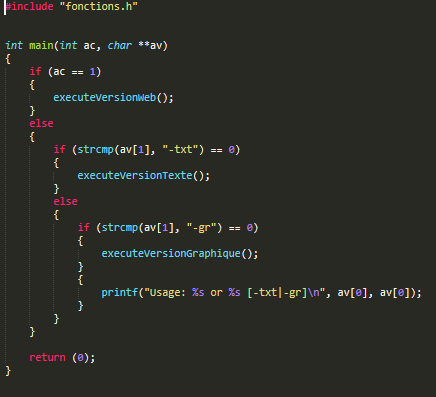
\includegraphics[width=0.6\textwidth]{MAINPOINTC.PNG}
  \caption{Code de main.c}
  \label{fig:courbe-tikz}
\end{figure}
\newpage 

Voici une capture d'écran du fichier "Fonction.c". En effet, pour éviter d'avoir à utiliser une structure de données représentant les 12 mois de l'année et, d'utiliser 12 if pour le traitement, nous avons fait une fonction \textbf{getIndex} qui permet de créer un tableau indexant tous les mois de l'année. De ce fait, pour chaque mois on pourra récupérer le nombre de connexions et effectuer un traitement.\\

La fonction \textbf{Decoupe$_$ligne} permet simplement de découper une ligne pour récupérer le mois et ensuite effectuer des traitements par dessus. 

\begin{figure}[htp!]
  \centering
  \setlength\figureheight{7cm}
  \setlength\figurewidth{9cm}
  \includegraphics[width=1\textwidth]{FONCTIONPOINTC1.PNG}
  \caption{Code de Fonction.c}
  \label{fig:courbe-tikz}
\end{figure}

\newpage

La fonction lecturestyle permet d'ouvrir le fichier de style html utile pour la version web. La fonction handleEvents est utilisé pour l'actualisation automatique de la version graphique. En effet, cette fonction permet de créer un listener sur le fichier de log et d'être notifié dès qu'il y a un changement dans ce fichier. De ce fait, dès qu'il y a eu une nouvelle requête sur le serveur, la version graphique du programme va se mettre à jour. Pour faire cette fonction, nous avons utilisé le man de la fonction inotify.

\begin{figure}[htp!]
  \centering
  \setlength\figureheight{7cm}
  \setlength\figurewidth{9cm}
  \includegraphics[width=1\textwidth]{FONCTIONPOINTC2.PNG}
  \caption{Code de Fonction.c}
  \label{fig:courbe-tikz}
\end{figure}

\newpage

La fonction monitorfile permet de pouvoir "écouter" le fichier acces.log et via la fonction handleEvents, d'être notifié à chaque changement. Pour la fonction versiontexte, nous avons compacté son code en utilisant une boucle for.

\begin{figure}[htp!]
  \centering
  \setlength\figureheight{7cm}  
  \setlength\figurewidth{9cm}
  \includegraphics[width=1.1\textwidth]{FONCTIONPOINTC3.PNG}
  \caption{Code de Fonction.c}
  \label{fig:courbe-tikz}
\end{figure}

\newpage

La fonction versionweb prend en paramètre deux floats retournés par la fonction stats que nous verrons après. Cette fonction fait simplement des printf de code html. De plus, comme mentionné plus haut, la fonction system(), permet de lancer un navigateur pour afficher le code web en cgi-bin.

\begin{figure}[htp!]
  \centering
  \setlength\figureheight{7cm}
  \setlength\figurewidth{9cm}
  \includegraphics[width=1\textwidth]{FONCTIONPOINTC4.PNG}
  \caption{Code de Fonction.c}
  \label{fig:courbe-tikz}
\end{figure}

\newpage

\begin{figure}[htp!]
  \centering
  \setlength\figureheight{7cm}
  \setlength\figurewidth{9cm}
  \includegraphics[width=1\textwidth]{FONCTIONPOINTC5.PNG}
  \caption{Code de Fonction.c}
  \label{fig:courbe-tikz}
\end{figure}


La fonction stats permet d'effectuer des calculs comme pour le nombre de connexions totales et le pourcentage pour chaque mois.

\begin{figure}[htp!]
  \centering
  \setlength\figureheight{7cm}
  \setlength\figurewidth{9cm}
  \includegraphics[width=0.7\textwidth]{FONCTIONPOINTC6.PNG}
  \caption{Code de Fonction.c}
  \label{fig:courbe-tikz}
\end{figure}

\newpage

Finalement, le fichier fonction.h ne contient que 3 prototypes, ce qui permet d'apporter un peu d'ordre dans notre code. 

\begin{figure}[htp!]
  \centering
  \setlength\figureheight{7cm}
  \setlength\figurewidth{9cm}
  \includegraphics[width=0.4\textwidth]{FONCTIONPOINTH.PNG}
  \caption{Code de Fonction.h}
  \label{fig:courbe-tikz}
\end{figure}